
%% bare_jrnl.tex
%% V1.4b
%% 2015/08/26
%% by Michael Shell
%% see http://www.michaelshell.org/
%% for current contact information.
%%
%% This is a skeleton file demonstrating the use of IEEEtran.cls
%% (requires IEEEtran.cls version 1.8b or later) with an IEEE
%% journal paper.
%%
%% Support sites:
%% http://www.michaelshell.org/tex/ieeetran/
%% http://www.ctan.org/pkg/ieeetran
%% and
%% http://www.ieee.org/

%%*************************************************************************
%% Legal Notice:
%% This code is offered as-is without any warranty either expressed or
%% implied; without even the implied warranty of MERCHANTABILITY or
%% FITNESS FOR A PARTICULAR PURPOSE! 
%% User assumes all risk.
%% In no event shall the IEEE or any contributor to this code be liable for
%% any damages or losses, including, but not limited to, incidental,
%% consequential, or any other damages, resulting from the use or misuse
%% of any information contained here.
%%
%% All comments are the opinions of their respective authors and are not
%% necessarily endorsed by the IEEE.
%%
%% This work is distributed under the LaTeX Project Public License (LPPL)
%% ( http://www.latex-project.org/ ) version 1.3, and may be freely used,
%% distributed and modified. A copy of the LPPL, version 1.3, is included
%% in the base LaTeX documentation of all distributions of LaTeX released
%% 2003/12/01 or later.
%% Retain all contribution notices and credits.
%% ** Modified files should be clearly indicated as such, including  **
%% ** renaming them and changing author support contact information. **
%%*************************************************************************


% *** Authors should verify (and, if needed, correct) their LaTeX system  ***
% *** with the testflow diagnostic prior to trusting their LaTeX platform ***
% *** with production work. The IEEE's font choices and paper sizes can   ***
% *** trigger bugs that do not appear when using other class files.       ***                          ***
% The testflow support page is at:
% http://www.michaelshell.org/tex/testflow/



\documentclass[journal]{IEEEtran}
%
% If IEEEtran.cls has not been installed into the LaTeX system files,
% manually specify the path to it like:
% \documentclass[journal]{../sty/IEEEtran}





% Some very useful LaTeX packages include:
% (uncomment the ones you want to load)


% *** MISC UTILITY PACKAGES ***
%
%\usepackage{ifpdf}
% Heiko Oberdiek's ifpdf.sty is very useful if you need conditional
% compilation based on whether the output is pdf or dvi.
% usage:
% \ifpdf
%   % pdf code
% \else
%   % dvi code
% \fi
% The latest version of ifpdf.sty can be obtained from:
% http://www.ctan.org/pkg/ifpdf
% Also, note that IEEEtran.cls V1.7 and later provides a builtin
% \ifCLASSINFOpdf conditional that works the same way.
% When switching from latex to pdflatex and vice-versa, the compiler may
% have to be run twice to clear warning/error messages.






% *** CITATION PACKAGES ***
%
\usepackage{cite}
% cite.sty was written by Donald Arseneau
% V1.6 and later of IEEEtran pre-defines the format of the cite.sty package
% \cite{} output to follow that of the IEEE. Loading the cite package will
% result in citation numbers being automatically sorted and properly
% "compressed/ranged". e.g., [1], [9], [2], [7], [5], [6] without using
% cite.sty will become [1], [2], [5]--[7], [9] using cite.sty. cite.sty's
% \cite will automatically add leading space, if needed. Use cite.sty's
% noadjust option (cite.sty V3.8 and later) if you want to turn this off
% such as if a citation ever needs to be enclosed in parenthesis.
% cite.sty is already installed on most LaTeX systems. Be sure and use
% version 5.0 (2009-03-20) and later if using hyperref.sty.
% The latest version can be obtained at:
% http://www.ctan.org/pkg/cite
% The documentation is contained in the cite.sty file itself.






% *** GRAPHICS RELATED PACKAGES ***
%
\ifCLASSINFOpdf
  \usepackage[pdftex]{graphicx}
  % declare the path(s) where your graphic files are
  \graphicspath{{./graphics/}}
  % and their extensions so you won't have to specify these with
  % every instance of \includegraphics
  \DeclareGraphicsExtensions{.pdf,.jpeg,.png}
\else
  % or other class option (dvipsone, dvipdf, if not using dvips). graphicx
  % will default to the driver specified in the system graphics.cfg if no
  % driver is specified.
  % \usepackage[dvips]{graphicx}
  % declare the path(s) where your graphic files are
  % \graphicspath{{../eps/}}
  % and their extensions so you won't have to specify these with
  % every instance of \includegraphics
  % \DeclareGraphicsExtensions{.eps}
\fi
% graphicx was written by David Carlisle and Sebastian Rahtz. It is
% required if you want graphics, photos, etc. graphicx.sty is already
% installed on most LaTeX systems. The latest version and documentation
% can be obtained at: 
% http://www.ctan.org/pkg/graphicx
% Another good source of documentation is "Using Imported Graphics in
% LaTeX2e" by Keith Reckdahl which can be found at:
% http://www.ctan.org/pkg/epslatex
%
% latex, and pdflatex in dvi mode, support graphics in encapsulated
% postscript (.eps) format. pdflatex in pdf mode supports graphics
% in .pdf, .jpeg, .png and .mps (metapost) formats. Users should ensure
% that all non-photo figures use a vector format (.eps, .pdf, .mps) and
% not a bitmapped formats (.jpeg, .png). The IEEE frowns on bitmapped formats
% which can result in "jaggedy"/blurry rendering of lines and letters as
% well as large increases in file sizes.
%
% You can find documentation about the pdfTeX application at:
% http://www.tug.org/applications/pdftex





% *** MATH PACKAGES ***
%
%\usepackage{amsmath}
% A popular package from the American Mathematical Society that provides
% many useful and powerful commands for dealing with mathematics.
%
% Note that the amsmath package sets \interdisplaylinepenalty to 10000
% thus preventing page breaks from occurring within multiline equations. Use:
%\interdisplaylinepenalty=2500
% after loading amsmath to restore such page breaks as IEEEtran.cls normally
% does. amsmath.sty is already installed on most LaTeX systems. The latest
% version and documentation can be obtained at:
% http://www.ctan.org/pkg/amsmath





% *** SPECIALIZED LIST PACKAGES ***
%
%\usepackage{algorithmic}
% algorithmic.sty was written by Peter Williams and Rogerio Brito.
% This package provides an algorithmic environment fo describing algorithms.
% You can use the algorithmic environment in-text or within a figure
% environment to provide for a floating algorithm. Do NOT use the algorithm
% floating environment provided by algorithm.sty (by the same authors) or
% algorithm2e.sty (by Christophe Fiorio) as the IEEE does not use dedicated
% algorithm float types and packages that provide these will not provide
% correct IEEE style captions. The latest version and documentation of
% algorithmic.sty can be obtained at:
% http://www.ctan.org/pkg/algorithms
% Also of interest may be the (relatively newer and more customizable)
% algorithmicx.sty package by Szasz Janos:
% http://www.ctan.org/pkg/algorithmicx




% *** ALIGNMENT PACKAGES ***
%
\usepackage{array}
% Frank Mittelbach's and David Carlisle's array.sty patches and improves
% the standard LaTeX2e array and tabular environments to provide better
% appearance and additional user controls. As the default LaTeX2e table
% generation code is lacking to the point of almost being broken with
% respect to the quality of the end results, all users are strongly
% advised to use an enhanced (at the very least that provided by array.sty)
% set of table tools. array.sty is already installed on most systems. The
% latest version and documentation can be obtained at:
% http://www.ctan.org/pkg/array


% IEEEtran contains the IEEEeqnarray family of commands that can be used to
% generate multiline equations as well as matrices, tables, etc., of high
% quality.




% *** SUBFIGURE PACKAGES ***
\ifCLASSOPTIONcompsoc
 \usepackage[caption=false,font=normalsize,labelfont=sf,textfont=sf]{subfig}
\else
 \usepackage[caption=false,font=footnotesize]{subfig}
\fi
% subfig.sty, written by Steven Douglas Cochran, is the modern replacement
% for subfigure.sty, the latter of which is no longer maintained and is
% incompatible with some LaTeX packages including fixltx2e. However,
% subfig.sty requires and automatically loads Axel Sommerfeldt's caption.sty
% which will override IEEEtran.cls' handling of captions and this will result
% in non-IEEE style figure/table captions. To prevent this problem, be sure
% and invoke subfig.sty's "caption=false" package option (available since
% subfig.sty version 1.3, 2005/06/28) as this is will preserve IEEEtran.cls
% handling of captions.
% Note that the Computer Society format requires a larger sans serif font
% than the serif footnote size font used in traditional IEEE formatting
% and thus the need to invoke different subfig.sty package options depending
% on whether compsoc mode has been enabled.
%
% The latest version and documentation of subfig.sty can be obtained at:
% http://www.ctan.org/pkg/subfig




% *** FLOAT PACKAGES ***
%
%\usepackage{fixltx2e}
% fixltx2e, the successor to the earlier fix2col.sty, was written by
% Frank Mittelbach and David Carlisle. This package corrects a few problems
% in the LaTeX2e kernel, the most notable of which is that in current
% LaTeX2e releases, the ordering of single and double column floats is not
% guaranteed to be preserved. Thus, an unpatched LaTeX2e can allow a
% single column figure to be placed prior to an earlier double column
% figure.
% Be aware that LaTeX2e kernels dated 2015 and later have fixltx2e.sty's
% corrections already built into the system in which case a warning will
% be issued if an attempt is made to load fixltx2e.sty as it is no longer
% needed.
% The latest version and documentation can be found at:
% http://www.ctan.org/pkg/fixltx2e


%\usepackage{stfloats}
% stfloats.sty was written by Sigitas Tolusis. This package gives LaTeX2e
% the ability to do double column floats at the bottom of the page as well
% as the top. (e.g., "\begin{figure*}[!b]" is not normally possible in
% LaTeX2e). It also provides a command:
%\fnbelowfloat
% to enable the placement of footnotes below bottom floats (the standard
% LaTeX2e kernel puts them above bottom floats). This is an invasive package
% which rewrites many portions of the LaTeX2e float routines. It may not work
% with other packages that modify the LaTeX2e float routines. The latest
% version and documentation can be obtained at:
% http://www.ctan.org/pkg/stfloats
% Do not use the stfloats baselinefloat ability as the IEEE does not allow
% \baselineskip to stretch. Authors submitting work to the IEEE should note
% that the IEEE rarely uses double column equations and that authors should try
% to avoid such use. Do not be tempted to use the cuted.sty or midfloat.sty
% packages (also by Sigitas Tolusis) as the IEEE does not format its papers in
% such ways.
% Do not attempt to use stfloats with fixltx2e as they are incompatible.
% Instead, use Morten Hogholm'a dblfloatfix which combines the features
% of both fixltx2e and stfloats:
%
% \usepackage{dblfloatfix}
% The latest version can be found at:
% http://www.ctan.org/pkg/dblfloatfix




%\ifCLASSOPTIONcaptionsoff
%  \usepackage[nomarkers]{endfloat}
% \let\MYoriglatexcaption\caption
% \renewcommand{\caption}[2][\relax]{\MYoriglatexcaption[#2]{#2}}
%\fi
% endfloat.sty was written by James Darrell McCauley, Jeff Goldberg and 
% Axel Sommerfeldt. This package may be useful when used in conjunction with 
% IEEEtran.cls'  captionsoff option. Some IEEE journals/societies require that
% submissions have lists of figures/tables at the end of the paper and that
% figures/tables without any captions are placed on a page by themselves at
% the end of the document. If needed, the draftcls IEEEtran class option or
% \CLASSINPUTbaselinestretch interface can be used to increase the line
% spacing as well. Be sure and use the nomarkers option of endfloat to
% prevent endfloat from "marking" where the figures would have been placed
% in the text. The two hack lines of code above are a slight modification of
% that suggested by in the endfloat docs (section 8.4.1) to ensure that
% the full captions always appear in the list of figures/tables - even if
% the user used the short optional argument of \caption[]{}.
% IEEE papers do not typically make use of \caption[]'s optional argument,
% so this should not be an issue. A similar trick can be used to disable
% captions of packages such as subfig.sty that lack options to turn off
% the subcaptions:
% For subfig.sty:
% \let\MYorigsubfloat\subfloat
% \renewcommand{\subfloat}[2][\relax]{\MYorigsubfloat[]{#2}}
% However, the above trick will not work if both optional arguments of
% the \subfloat command are used. Furthermore, there needs to be a
% description of each subfigure *somewhere* and endfloat does not add
% subfigure captions to its list of figures. Thus, the best approach is to
% avoid the use of subfigure captions (many IEEE journals avoid them anyway)
% and instead reference/explain all the subfigures within the main caption.
% The latest version of endfloat.sty and its documentation can obtained at:
% http://www.ctan.org/pkg/endfloat
%
% The IEEEtran \ifCLASSOPTIONcaptionsoff conditional can also be used
% later in the document, say, to conditionally put the References on a 
% page by themselves.




% *** PDF, URL AND HYPERLINK PACKAGES ***
%
\usepackage{url}
% url.sty was written by Donald Arseneau. It provides better support for
% handling and breaking URLs. url.sty is already installed on most LaTeX
% systems. The latest version and documentation can be obtained at:
% http://www.ctan.org/pkg/url
% Basically, \url{my_url_here}.




% *** Do not adjust lengths that control margins, column widths, etc. ***
% *** Do not use packages that alter fonts (such as pslatex).         ***
% There should be no need to do such things with IEEEtran.cls V1.6 and later.
% (Unless specifically asked to do so by the journal or conference you plan
% to submit to, of course. )

% correct bad hyphenation here
\hyphenation{op-tical net-works semi-conduc-tor}


\begin{document}
%
% paper title
% Titles are generally capitalized except for words such as a, an, and, as,
% at, but, by, for, in, nor, of, on, or, the, to and up, which are usually
% not capitalized unless they are the first or last word of the title.
% Linebreaks \\ can be used within to get better formatting as desired.
% Do not put math or special symbols in the title.
\title{Keyshuffling Attack for Persistent Early Code Execution in the Nintendo
3DS Secure Bootchain}
%
%
% author names and IEEE memberships
% note positions of commas and nonbreaking spaces ( ~ ) LaTeX will not break
% a structure at a ~ so this keeps an author's name from being broken across
% two lines.
% use \thanks{} to gain access to the first footnote area
% a separate \thanks must be used for each paragraph as LaTeX2e's \thanks
% was not built to handle multiple paragraphs
%

\author{Devon~"Plailect"~Maloney, "stuckpixel", "SciresM", "Gelex", "Normmatt", and~"Aurora~Wright"\vspace{-2.0em}}

% note the % following the last \IEEEmembership and also \thanks - 
% these prevent an unwanted space from occurring between the last author name
% and the end of the author line. i.e., if you had this:
% 
% \author{....lastname \thanks{...} \thanks{...} }
%                     ^------------^------------^----Do not want these spaces!
%
% a space would be appended to the last name and could cause every name on that
% line to be shifted left slightly. This is one of those "LaTeX things". For
% instance, "\textbf{A} \textbf{B}" will typeset as "A B" not "AB". To get
% "AB" then you have to do: "\textbf{A}\textbf{B}"
% \thanks is no different in this regard, so shield the last } of each \thanks
% that ends a line with a % and do not let a space in before the next \thanks.
% Spaces after \IEEEmembership other than the last one are OK (and needed) as
% you are supposed to have spaces between the names. For what it is worth,
% this is a minor point as most people would not even notice if the said evil
% space somehow managed to creep in.

% make the title area
\maketitle

% As a general rule, do not put math, special symbols or citations
% in the abstract or keywords.
\begin{abstract}
We demonstrate an attack on the secure bootchain of the Nintendo 3DS in order to
gain early code execution. The attack utilizes the block shuffling vulnerability
of the ECB cipher mode to rearrange keys in the Nintendo 3DS's encrypted
keystore. Because the shuffled keys will deterministically decrypt the encrypted
firmware binary to incorrect plaintext data and execute it, and because the
device's memory contents are kept between hard reboots, it is possible to
reliably reach a branching instruction to a payload in memory. This payload, due
to its execution by a privileged processor and its early execution, is able to
extract the hash of hardware secrets necessary to decrypt the device's encrypted
keystore and set up a persistant exploit of the system.
\end{abstract}

\begin{IEEEkeywords}
Advanced Encryption Standard, keyshuffling, bootchain, cryptography, block
ciphers, software security.
\end{IEEEkeywords}

\section{Introduction}

The Nintendo 3DS, like all entertainment consoles, is in a difficult position
when it comes to designing a secure system. The device must easily accommodate
legitimate users while at the same time preventing cheating, protecting
intellectual property, and enforcing system integrity. To accomplish this, the
3DS has a chain of trust based on two separate processors: an ARM9 and an ARM11.
The ARM9 processor is a security processor that runs a single process
("Process9") whose sole responsibility is to handle secure functions such as
cryptography, filesystem access, and permissions. The ARM11 processor is an
application processor that which is reponsible for all OS and userspace-level
tasks \cite{cryptosystem}.

As with most embedded systems, the root of trust for the 3DS is the boot ROM
burned into the System-on-Chip ("SoC") at the factory. The code in this Read
Only Memory cannot be changed and contains a public key to which only Nintendo
has the matching private key. When the device is powered on, each CPU's boot ROM
loads their respective firmware binary from NAND flash storage to memory, checks
the firmware binary for a valid RSA signature that matches the burned in public
key, then jumps to the firmware binary entrypoint \cite{cryptosystem}. This is a
simple, robust chain of trust that seems fairly secure upon initial inspection.

In 2014, Nintendo released the "New 3DS" which this paper will focus on. This
updated 3DS features a faster CPU, more RAM, and (most importantly) an extra
encryption layer on the ARM9 firmware binary known in the 3DS community as
"ARM9Loader". This encryption layer loads new keys from NAND sector 0x96 (the
plaintext of which is the same for all New 3DS devices), which are encrypted
with AES-128-ECB by a key calculated from a SHA-256 hash of the the
console-unique (different for every console) "OTP" memory region of the device.
Keys on the 3DS are loaded into write-only "keyslots", which are secure memory
areas readable only by the hardware AES implementation. This means that it
should not be possible to recover these keys after they have been written to the
AES module \cite{AES_Registers}.

After ARM9Loader decrypts the NAND "keysector", access to the OTP memory region
is disabled until next boot via the hardware register CFG\_SYSPROT9. Once the
OTP region has been secured, ARM9Loader then decrypts the ARM9 firmware binary
using a key from the decryted keysector. Additionally, the hash of the OTP
memory region is outputted to the SHA\_HASH hardware register after the hardware
SHA implementation calculates it \cite{SHA_Registers}. Importantly, This
register is not cleared until the ARM9 firmware binary clears it after
ARM9Loader jumps to its entrypoint.

\section{Secure Bootchain Implementations}

\subsection{Implementation (v1.0)}

The New 3DS shipped with version 8.1.0 of the system software, which contains
the following implementation of ARM9Loader in the boot process \cite{FIRM}:

\medskip
\begin{enumerate}
  \item Calculate SHA-256 hash of the OTP memory region and output the hash to
  the SHA\_HASH register
  \item Calculate AES write-only keyslot 0x11 from the OTP hash
  \item Read the keysector from NAND to memory
  \item Decrypt the keysector using keyslot 0x11
  \item Clear AES write-only keyslot 0x11 to zero
  \item Disable access to the OTP memory region by setting CFG\_SYSPROT9
  \item Write Key \#1 from the keysector to AES write-only keyslot 0x11
  \item Instruct the AES module to calculate sub-keys 0x18 through 0x1F based on
  keyslot 0x11
  \item Verify keyslot 0x11 by encrypting a fixed test vector and checking the
  result
  \item Instruct the AES module to decrypt the ARM9 firmware binary
  \item Jump to the ARM9 firmware binary entrypoint
\end{enumerate}
\medskip

The problem with this implementation of ARM9Loader is that keyslot 0x11 was not
cleared after decrypting the ARM9 firmware binary (before jumping to the
entrypoint), and thus it was possible to gain ARM9 code execution at a later
point and instruct the AES module to regenerate all of the secret sub-keys
without having access to the decrypted keysector. This was partially fixed with
the update 9.5.0 by clearing keyslot 0x11 after ARM9Loader decrypts the ARM9
firmware binary, but keyslot 0x11 was still set with keysector Key \#1
\cite{3DS_System_Flaws}.

\subsection{Implementation (v2.0)}

The system software update 9.6.0 fixed the shortcomings of the first ARM9Loader
implementation by using a different keysector key and clearing it properly this
time. It contains the following implementation of ARM9Loader in the boot process
\cite{FIRM}:

\medskip
\begin{enumerate}
  \item Calculate SHA-256 hash of the OTP memory region and output the hash to
  the SHA\_HASH register
  \item Calculate AES write-only keyslot 0x11 from the OTP hash
  \item Read the keysector from NAND to memory
  \item Decrypt the keysector using keyslot 0x11
  \item Clear AES write-only keyslot 0x11 to zero
  \item Disable access to the OTP memory region by setting CFG\_SYSPROT9
  \item Decrypt a key from within ARM9Loader's read-only data and set that key
  to keyslot 0x18
  \item Write Key \#1 from the keysector to AES write-only keyslot 0x11
  \item Instruct the AES module to calculate sub-keys 0x19 through 0x1F based on
  keyslot 0x11
  \item Verify keyslot 0x11 by encrypting a fixed test vector and checking the
  result
  \item Write Key \#2 from the keysector to AES write-only keyslot 0x11
  \item Instruct the AES module to decrypt the ARM9 firmware binary
  \item Disable access to the OTP memory region by setting CFG\_SYSPROT9
  \item Clear AES write-only keyslot 0x11 to zero
  \item Jump to the ARM9 firmware binary entrypoint
\end{enumerate}
\medskip

The problem with this implementation of ARM9Loader is that Key \#2 is never
verified by encrypting a fixed test vector and checking the result, meaning that
Key \#2 can be altered and the ARM9 firmware binary will be deterministically
decrypted to incorrect plaintext data and executed. Unfortunately, because the
keysector is encrypted with the console unique OTP hash (which we cannot access
post-ARM9Loader), it is not possible to arbitrarily write any key to it and get
a predictable decryption result \cite{3DS_System_Flaws}.

\section{Keyshuffling}

The keysector is encrypted with AES-128-ECB, where AES is the encryption
standard, 128 is the number of bits in a block, and ECB is the cipher mode. The
two parts of this specific encryption method that interest us are the block size
and the cipher mode. The keys in the keysector are all 16 bytes (128 bits) long,
and there is no message authentication code of any kind to increase the size or
validate the key positions. This is a crucial fact because of the cipher mode
used. In Electronic Codebook (ECB), each block in the message (the keysector in
this case) is divided into blocks of the given size and encrypted separately.
This means that each key in the keysector aligns with a block that is encrypted
completely separately from all of the other aligned keys, allowing us to move
the keys into any position we want while still decrypting properly.

Another critical aspect of this attack is that each version of the ARM9 firmware
binary is encrypted with a different counter in AES-128-CTR mode, meaning that
even code that is the same between versions will decrypt to something completely
different for each key that we try. A NAND sector on the device is 0x200 bytes
and each key is 0x10 bytes. When we do not count the Key \#2 that properly
decrypts the ARM9 firmware binary, that means we have 31 different keys for each
ARM9 firmware binary version that will all decrypt the binary to a different
incorrect plaintext which will then be executed.

\begin{figure}[h]
  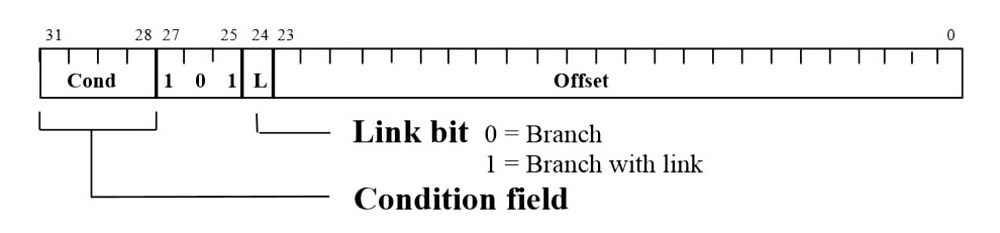
\includegraphics[width=\columnwidth]{./images/branchinstruction.jpg}
  \caption{Encoding of an ARM branch instruction \cite{32c3}}
\end{figure}

If we try enough keys and ARM9 firmware binary versions, there is a high
probability that we will eventually find one that decrypts the ARM9 firmware
binary deterministically such that the entrypoint is a branch instruction to
another memory address where a payload can be placed. We found, by trying all
possible keys and ARM9 firmware binary versions, that there is one combination
that causes a jump to a usable memory location. By installing the 10.0.0 update
of the ARM9 firmware binary and using the keyshuffling attack to replace
keysector Key \#2 with a copy of keysector Key \#1, the resulting incorrect
plaintext from the deterministic decryption will have a jump to memory address
\texttt{0x80FD0F8} at the ARM9 firmware binary entrypoint. This redirects the
code flow outside of the secure bootchain and into manipulatable memory.

To exploit this vulnerable redirection of code flow, we took advantage of
another major oversight in the device's design: when the device reboots, all
memory keeps its contents. This makes it possible for us to gain ARM9 code
execution at a point after the system boot completes, install the 10.0.0 update
of the ARM9 firmware binary, use keyshuffling to replace keysector Key \#2 with
keysector Key \#1, insert a series of NOP instructions ("NOP sled") at memory
address 0x80FD0F8 followed by a payload that dumps the SHA\_HASH register, then
reboot.

When the device comes back up, the ARM9 boot ROM will read ARM9Loader and the
encrypted ARM9 firmware binary to memory, then jump to ARM9Loader which will
perform the implementation v2.0 steps described previously. ARM9Loader will then
(incorrectly) attempts to decrypt the ARM9 firmware with Key \#2 (which is now
identical to Key \#1), disable access to the OTP memory region by setting
CFG\_SYSPROT9, and jump to the ARM9 firmware binary entrypoint. When it does, it
will immediately jump to memory address \texttt{0x80FD0F8}, execute the series
of NOP instructions and "slide" to the payload. The payload then copies the
hash of the OTP memory region from the uncleared SHA\_HASH output register for
the purpose of decrypting the keysector at a later point.

\section{Persistence}

With the SHA-256 hash of the OTP memory region, we are now able to decrypt or
re-encrypt the keysector. This means that we now completely control what key
will be used for decrypting the ARM9 firmware binary, rather than being limited
to one of the other 31 keys in the keysector. To understand how controlling the
location of memory jumped to by ARM9Loader is useful in the context of
persistence, we must look at how the boot ROM loads ARM9Loader and the firmware
binary from NAND to memory.

On the 3DS, ARM9Loader and the ARM9 Firmware binary, known collectively as
"FIRM", are stored twice on NAND in two partitions known as "FIRM0" and "FIRM1
for redundancy purposes. This means that if one firmware partition becomes
corrupted, the device will still boot. Note that the FIRM partitions, as with
most partitions on the device, are encrypted using console unique keys derrved
from the OTP and set by the bootrom. The boot ROM uses the following
implementation to load FIRM0 and FIRM1 from NAND
\cite{clevermind}\cite{Bootloader}\cite{OTP_Registers}:

\medskip
\begin{enumerate}
  \item Decrypt the OTP memory region and store the first 0x90 bytes in
  Instruction Tightly-Coupled Memory ("ITCM")\cite{OTP_Registers}
  \item Calculate AES write-only keyslot 0x06 from decrypted OTP memory region
  in ITCM
  \item Read FIRM0 NAND partition to memory
  \item Decrypt FIRM0 partition in memory using keyslot 0x06
  \item Check the RSA signature of decrypted FIRM0 against burned in public key
    \begin{enumerate}
    \item If the RSA signature is valid, jump to FIRM0 ARM9Loader entrypoint
    \item If the RSA signature is invalid, continue
    \end{enumerate}
  \item Read FIRM1 NAND partition to memory on top of FIRM0
  \item Decrypt FIRM1 partition in memory using keyslot 0x06
  \item Check the RSA signature of decrypted FIRM1 against burned in public key
    \begin{enumerate}
    \item If the RSA signature is valid, jump to FIRM1 ARM9Loader entrypoint
    \item If the RSA signature is invalid, panic
    \end{enumerate}
\end{enumerate}
\medskip

The problem with this implementation is that, in the case of a FIRM0 partition
with an invalid signature, FIRM1 is loaded on top of it without FIRM0's memory
being cleared \cite{32c3}. This allows for an attack in which we install the
largest legitimately signed ARM9 firmware binary available to us (8.1.0) into
FIRM0, then install the smallest legitimately signed ARM9 firmware binary
available to us (10.2.0) into FIRM1. We could then place a payload of our
choosing on top of FIRM0 at a point after FIRM1's size and find a key whose
deterministic decryption of the 10.2.0 ARM9 firmware binary to a resulting
incorrect plaintext will have a branch instruction to memory address after the
end of the 10.2.0 ARM9 firmware binary but within the size of the 8.1.0 ARM9
firmware binary \cite{32c3}.

We ran a bruteforce of all possible Key \#2 values until we found the key whose
deterministic decryption of the 8.1.0 FIRM0 ARM9 firmware binary to a resulting
incorrect plaintext has a branch instruction to 0x190 bytes after the end of the
8.1.0 ARM9 firmware binary (\texttt{0x0824D3CB4AE94D624DAA526047C59394}). We use
0x190 bytes after the end of the 8.1.0 ARM9 firmware binary because empirical
tests determined that placing the payload any sooner after the 8.1.0 ARM9
firmware binary caused the payload to be overwritten by an unknown factor in the
boot process (likely the stack or bss segment). After finding this key, we
encrypt it with the OTP memory region hash obtained through the keyshuffling
exploit and install the encrypted key into keysector Key \#2. We then add 0x190
to the size of the 8.1.0 ARM9 firmware binary and write a payload of our
choosing to that position relative to the 10.2.0 ARM9 firmware binary
\cite{32c3}.

When the device is rebooted, the boot ROM loads FIRM0 into memory and decrypts
it with AES write-only keyslot 0x06. It then checks the RSA signature of
decrypted FIRM0, which fails because our payload at the end of the 8.1.0 ARM9
firmware binary has modified the hash. The boot ROM then, without clearing the
memory now containing our payload, loads FIRM1 into memory on top of FIRM0 and
decrypts it with AES write-only keyslot 0x06 \cite{clevermind}. The boot ROM
checks the RSA signature of FIRM1, which passes because the payload comes after
the 10.2.0 ARM9 firmware binary. The boot ROM then jumps to the FIRM1 ARM9Loader
in memory which uses our crafted Key \#2 to deterministically decrypt the 8.1.0
ARM9 firmware binary to an incorrect plaintext and jumps to its entrypoint. When
it does, it will immediately jump to the memory address of the payload of our
choosing, giving us ARM9 code execution on every successive boot before the ARM9
firmware binary runs \cite{32c3}\cite{clevermind}.

\section{Conclusion}

We have demonstrated a keyshuffling attack on the secure bootchain of the
Nintendo 3DS in order to redirect code flow into insecure memory. This allowed
us to gain code execution early enough to extract hardware secrets for the
purpose of setting up persistent early code execution that survives reboots.
This attack was made possible through a hardware revision that included the
addition of a new encryption layer that not only failed to provide extra
security, but additionally compromised a bootchain which had previously been
considered secure. This shows the danger of including new security measures in
an existing chain of trust without properly vetting them.

%\section*{Acknowledgment}

% references section

% can use a bibliography generated by BibTeX as a .bbl file
% BibTeX documentation can be easily obtained at:
% http://mirror.ctan.org/biblio/bibtex/contrib/doc/
% The IEEEtran BibTeX style support page is at:
% http://www.michaelshell.org/tex/ieeetran/bibtex/
\bibliographystyle{IEEEtran.bst}
\bibliography{IEEEabrv,references}
%
% <OR> manually copy in the resultant .bbl file
% set second argument of \begin to the number of references
% (used to reserve space for the reference number labels box)
%\begin{thebibliography}{1}

% \bibitem{IEEEhowto:kopka}
% H.~Kopka and P.~W. Daly, \emph{A Guide to \LaTeX}, 3rd~ed.\hskip 1em plus
%   0.5em minus 0.4em\relax Harlow, England: Addison-Wesley, 1999.

% \end{thebibliography}

% that's all folks
\end{document}


